% Options for packages loaded elsewhere
\PassOptionsToPackage{unicode}{hyperref}
\PassOptionsToPackage{hyphens}{url}
\PassOptionsToPackage{dvipsnames,svgnames,x11names}{xcolor}
%
\documentclass[
  letterpaper,
  DIV=11,
  numbers=noendperiod]{scrartcl}

\usepackage{amsmath,amssymb}
\usepackage{iftex}
\ifPDFTeX
  \usepackage[T1]{fontenc}
  \usepackage[utf8]{inputenc}
  \usepackage{textcomp} % provide euro and other symbols
\else % if luatex or xetex
  \usepackage{unicode-math}
  \defaultfontfeatures{Scale=MatchLowercase}
  \defaultfontfeatures[\rmfamily]{Ligatures=TeX,Scale=1}
\fi
\usepackage{lmodern}
\ifPDFTeX\else  
    % xetex/luatex font selection
\fi
% Use upquote if available, for straight quotes in verbatim environments
\IfFileExists{upquote.sty}{\usepackage{upquote}}{}
\IfFileExists{microtype.sty}{% use microtype if available
  \usepackage[]{microtype}
  \UseMicrotypeSet[protrusion]{basicmath} % disable protrusion for tt fonts
}{}
\makeatletter
\@ifundefined{KOMAClassName}{% if non-KOMA class
  \IfFileExists{parskip.sty}{%
    \usepackage{parskip}
  }{% else
    \setlength{\parindent}{0pt}
    \setlength{\parskip}{6pt plus 2pt minus 1pt}}
}{% if KOMA class
  \KOMAoptions{parskip=half}}
\makeatother
\usepackage{xcolor}
\setlength{\emergencystretch}{3em} % prevent overfull lines
\setcounter{secnumdepth}{-\maxdimen} % remove section numbering
% Make \paragraph and \subparagraph free-standing
\ifx\paragraph\undefined\else
  \let\oldparagraph\paragraph
  \renewcommand{\paragraph}[1]{\oldparagraph{#1}\mbox{}}
\fi
\ifx\subparagraph\undefined\else
  \let\oldsubparagraph\subparagraph
  \renewcommand{\subparagraph}[1]{\oldsubparagraph{#1}\mbox{}}
\fi

\usepackage{color}
\usepackage{fancyvrb}
\newcommand{\VerbBar}{|}
\newcommand{\VERB}{\Verb[commandchars=\\\{\}]}
\DefineVerbatimEnvironment{Highlighting}{Verbatim}{commandchars=\\\{\}}
% Add ',fontsize=\small' for more characters per line
\usepackage{framed}
\definecolor{shadecolor}{RGB}{241,243,245}
\newenvironment{Shaded}{\begin{snugshade}}{\end{snugshade}}
\newcommand{\AlertTok}[1]{\textcolor[rgb]{0.68,0.00,0.00}{#1}}
\newcommand{\AnnotationTok}[1]{\textcolor[rgb]{0.37,0.37,0.37}{#1}}
\newcommand{\AttributeTok}[1]{\textcolor[rgb]{0.40,0.45,0.13}{#1}}
\newcommand{\BaseNTok}[1]{\textcolor[rgb]{0.68,0.00,0.00}{#1}}
\newcommand{\BuiltInTok}[1]{\textcolor[rgb]{0.00,0.23,0.31}{#1}}
\newcommand{\CharTok}[1]{\textcolor[rgb]{0.13,0.47,0.30}{#1}}
\newcommand{\CommentTok}[1]{\textcolor[rgb]{0.37,0.37,0.37}{#1}}
\newcommand{\CommentVarTok}[1]{\textcolor[rgb]{0.37,0.37,0.37}{\textit{#1}}}
\newcommand{\ConstantTok}[1]{\textcolor[rgb]{0.56,0.35,0.01}{#1}}
\newcommand{\ControlFlowTok}[1]{\textcolor[rgb]{0.00,0.23,0.31}{#1}}
\newcommand{\DataTypeTok}[1]{\textcolor[rgb]{0.68,0.00,0.00}{#1}}
\newcommand{\DecValTok}[1]{\textcolor[rgb]{0.68,0.00,0.00}{#1}}
\newcommand{\DocumentationTok}[1]{\textcolor[rgb]{0.37,0.37,0.37}{\textit{#1}}}
\newcommand{\ErrorTok}[1]{\textcolor[rgb]{0.68,0.00,0.00}{#1}}
\newcommand{\ExtensionTok}[1]{\textcolor[rgb]{0.00,0.23,0.31}{#1}}
\newcommand{\FloatTok}[1]{\textcolor[rgb]{0.68,0.00,0.00}{#1}}
\newcommand{\FunctionTok}[1]{\textcolor[rgb]{0.28,0.35,0.67}{#1}}
\newcommand{\ImportTok}[1]{\textcolor[rgb]{0.00,0.46,0.62}{#1}}
\newcommand{\InformationTok}[1]{\textcolor[rgb]{0.37,0.37,0.37}{#1}}
\newcommand{\KeywordTok}[1]{\textcolor[rgb]{0.00,0.23,0.31}{#1}}
\newcommand{\NormalTok}[1]{\textcolor[rgb]{0.00,0.23,0.31}{#1}}
\newcommand{\OperatorTok}[1]{\textcolor[rgb]{0.37,0.37,0.37}{#1}}
\newcommand{\OtherTok}[1]{\textcolor[rgb]{0.00,0.23,0.31}{#1}}
\newcommand{\PreprocessorTok}[1]{\textcolor[rgb]{0.68,0.00,0.00}{#1}}
\newcommand{\RegionMarkerTok}[1]{\textcolor[rgb]{0.00,0.23,0.31}{#1}}
\newcommand{\SpecialCharTok}[1]{\textcolor[rgb]{0.37,0.37,0.37}{#1}}
\newcommand{\SpecialStringTok}[1]{\textcolor[rgb]{0.13,0.47,0.30}{#1}}
\newcommand{\StringTok}[1]{\textcolor[rgb]{0.13,0.47,0.30}{#1}}
\newcommand{\VariableTok}[1]{\textcolor[rgb]{0.07,0.07,0.07}{#1}}
\newcommand{\VerbatimStringTok}[1]{\textcolor[rgb]{0.13,0.47,0.30}{#1}}
\newcommand{\WarningTok}[1]{\textcolor[rgb]{0.37,0.37,0.37}{\textit{#1}}}

\providecommand{\tightlist}{%
  \setlength{\itemsep}{0pt}\setlength{\parskip}{0pt}}\usepackage{longtable,booktabs,array}
\usepackage{calc} % for calculating minipage widths
% Correct order of tables after \paragraph or \subparagraph
\usepackage{etoolbox}
\makeatletter
\patchcmd\longtable{\par}{\if@noskipsec\mbox{}\fi\par}{}{}
\makeatother
% Allow footnotes in longtable head/foot
\IfFileExists{footnotehyper.sty}{\usepackage{footnotehyper}}{\usepackage{footnote}}
\makesavenoteenv{longtable}
\usepackage{graphicx}
\makeatletter
\def\maxwidth{\ifdim\Gin@nat@width>\linewidth\linewidth\else\Gin@nat@width\fi}
\def\maxheight{\ifdim\Gin@nat@height>\textheight\textheight\else\Gin@nat@height\fi}
\makeatother
% Scale images if necessary, so that they will not overflow the page
% margins by default, and it is still possible to overwrite the defaults
% using explicit options in \includegraphics[width, height, ...]{}
\setkeys{Gin}{width=\maxwidth,height=\maxheight,keepaspectratio}
% Set default figure placement to htbp
\makeatletter
\def\fps@figure{htbp}
\makeatother

\KOMAoption{captions}{tableheading}
\makeatletter
\makeatother
\makeatletter
\makeatother
\makeatletter
\@ifpackageloaded{caption}{}{\usepackage{caption}}
\AtBeginDocument{%
\ifdefined\contentsname
  \renewcommand*\contentsname{Tabla de contenidos}
\else
  \newcommand\contentsname{Tabla de contenidos}
\fi
\ifdefined\listfigurename
  \renewcommand*\listfigurename{Listado de Figuras}
\else
  \newcommand\listfigurename{Listado de Figuras}
\fi
\ifdefined\listtablename
  \renewcommand*\listtablename{Listado de Tablas}
\else
  \newcommand\listtablename{Listado de Tablas}
\fi
\ifdefined\figurename
  \renewcommand*\figurename{Figura}
\else
  \newcommand\figurename{Figura}
\fi
\ifdefined\tablename
  \renewcommand*\tablename{Tabla}
\else
  \newcommand\tablename{Tabla}
\fi
}
\@ifpackageloaded{float}{}{\usepackage{float}}
\floatstyle{ruled}
\@ifundefined{c@chapter}{\newfloat{codelisting}{h}{lop}}{\newfloat{codelisting}{h}{lop}[chapter]}
\floatname{codelisting}{Listado}
\newcommand*\listoflistings{\listof{codelisting}{Listado de Listados}}
\makeatother
\makeatletter
\@ifpackageloaded{caption}{}{\usepackage{caption}}
\@ifpackageloaded{subcaption}{}{\usepackage{subcaption}}
\makeatother
\makeatletter
\@ifpackageloaded{tcolorbox}{}{\usepackage[skins,breakable]{tcolorbox}}
\makeatother
\makeatletter
\@ifundefined{shadecolor}{\definecolor{shadecolor}{rgb}{.97, .97, .97}}
\makeatother
\makeatletter
\makeatother
\makeatletter
\makeatother
\ifLuaTeX
\usepackage[bidi=basic]{babel}
\else
\usepackage[bidi=default]{babel}
\fi
\babelprovide[main,import]{spanish}
% get rid of language-specific shorthands (see #6817):
\let\LanguageShortHands\languageshorthands
\def\languageshorthands#1{}
\ifLuaTeX
  \usepackage{selnolig}  % disable illegal ligatures
\fi
\IfFileExists{bookmark.sty}{\usepackage{bookmark}}{\usepackage{hyperref}}
\IfFileExists{xurl.sty}{\usepackage{xurl}}{} % add URL line breaks if available
\urlstyle{same} % disable monospaced font for URLs
\hypersetup{
  pdftitle={Tarea 1},
  pdflang={es},
  colorlinks=true,
  linkcolor={blue},
  filecolor={Maroon},
  citecolor={Blue},
  urlcolor={Blue},
  pdfcreator={LaTeX via pandoc}}

\title{Tarea 1}
\author{}
\date{}

\begin{document}
\maketitle
\ifdefined\Shaded\renewenvironment{Shaded}{\begin{tcolorbox}[boxrule=0pt, enhanced, breakable, sharp corners, interior hidden, borderline west={3pt}{0pt}{shadecolor}, frame hidden]}{\end{tcolorbox}}\fi

\hypertarget{respuestas}{%
\subsection{Respuestas}\label{respuestas}}

Cargamos paquetes

\begin{Shaded}
\begin{Highlighting}[]
\NormalTok{knitr}\SpecialCharTok{::}\NormalTok{opts\_chunk}\SpecialCharTok{$}\FunctionTok{set}\NormalTok{(}\AttributeTok{echo =} \ConstantTok{FALSE}\NormalTok{,}
                      \AttributeTok{warning =} \ConstantTok{FALSE}\NormalTok{,}
                      \AttributeTok{message =} \ConstantTok{FALSE}\NormalTok{)}
\FunctionTok{library}\NormalTok{(tidyverse)}
\FunctionTok{library}\NormalTok{(knitr)}
\FunctionTok{library}\NormalTok{(stargazer)}
\FunctionTok{library}\NormalTok{(janitor)}
\FunctionTok{library}\NormalTok{(sandwich)}
\FunctionTok{library}\NormalTok{(nnet)}
\FunctionTok{library}\NormalTok{(marginaleffects)}
\end{Highlighting}
\end{Shaded}

\hypertarget{pregunta-1}{%
\subsection{Pregunta 1}\label{pregunta-1}}

Suponga que está interesado en una variable aleatoria que tiene una
distribución Bernoulli con parámetro \(p\). La función de densidad está
definida como:

\[f(x_;p)=\left\{\begin{array} .1 & \text{con probabilidad } p \\ 0 & \text{con probabilidad } 1-p \end{array} \right.\]
Suponga que tiene una muestra de \(N\) observaciones independientes e
idénticamente distribuidas.

\begin{enumerate}
\def\labelenumi{\alph{enumi}.}
\item
  {[}4 puntos{]} Plantee la función de log verosimilitud del problema.
\item
  {[}4 puntos{]} Obtenga las condiciones de primer orden y resuelva para
  \(\hat{p}\).
\item
  {[}2 puntos{]} ¿Cuál es la media y la varianza del estimador de máxima
  verosimilitud que ha encontrado?
\end{enumerate}

\hypertarget{pregunta-2}{%
\subsection{Pregunta 2}\label{pregunta-2}}

Suponga que
\(y_i|\mathbf{x}_i\sim\mathcal{N}(m(\mathbf{x}_i,\mathbf{\beta}_0),\sigma_0^2)\),
donde \(m(\mathbf{x},\mathbf{\beta})\) es una función del vector de
variables explicativas \(\mathbf{x}\) y del vector de parámetros
\(\mathbf{\beta}\) de dimensión \((k\times 1)\). Entonces,
\(E(y_i|\mathbf{x}_i)=m(\mathbf{x}_i,\mathbf{\beta}_0)\) y
\(V(y_i|\mathbf{x}_i)=\sigma^2_0\).

\begin{enumerate}
\def\labelenumi{\alph{enumi}.}
\item
  {[}2 puntos{]} Escriba la función de log verosimilitud condicional
  para la observación \(i\). Muestre que el estimador de máxima
  verosimilitud \(\hat{\mathbf{\beta}}\) resuelve el problema de
  minimización
  \(\min_\mathbf{\beta}\sum_i(y_i-m(\mathbf{x}_i,\mathbf{\beta}))^2\).
\item
  {[}4 puntos{]} Sea
  \(\mathbf{\theta}\equiv(\mathbf{\beta}'\;\sigma^2)'\) un vector de
  parámetros de dimensión \((k+1)\times 1\). Encuentre el vector score
  para la observación \(i\). Muestre que
  \(E(\mathbf{s}_i(\mathbf{\theta}_0)|\mathbf{x}_i)=\mathbf{0}\).
\item
  {[}2 puntos{]} Usando las condiciones de primer orden, encuentre
  \(\hat{\sigma}^2\) en términos de \(\hat{\mathbf{\beta}}\).
\item
  {[}5 puntos{]} Encuentre la matriz hesiana de la función de log
  verosimilitud con respecto a \(\mathbf{\theta}\).
\item
  {[}5 puntos{]} Muestre que
  \(-E(\mathbf{H}_i(\mathbf{\theta}_0)|\mathbf{x}_i)=E(\mathbf{s}_i(\mathbf{\theta}_0)\mathbf{s}_i(\mathbf{\theta}_0)'|\mathbf{x}_i)\).
\item
  {[}2 puntos{]} Encuentre la varianza asintótica estimada de
  \(\hat{\mathbf{\beta}}\) y explique cómo obtendría los errores
  estándar.
\end{enumerate}

\hypertarget{pregunta-3}{%
\subsection{Pregunta 3}\label{pregunta-3}}

Suponga una variable aleatoria \(X_i\) con distribución desconocida. Sin
embargo, sí conocemos que \(E(X)=\mu=54\) y que
\(\sqrt{V(X)}=\sigma=6\). Suponga que se recolecta una muestra de 50
observaciones.

\begin{enumerate}
\def\labelenumi{\alph{enumi}.}
\item
  {[}2 punto{]} ¿Cuál es la distribución asintótica de la media muestral
  \(\bar{X}\)?
\item
  {[}4 punto{]} ¿Cuál es la probabilidad de que \(\bar{X}>58\)?
\item
  {[}2 punto{]} ¿Cuál es la probabilidad de que una observación elegida
  al azar sea tal que \(X_i>58\)?
\item
  {[}2 punto{]} Provea un intervalo de confianza de 99\% para la media
  muestral.
\end{enumerate}

\hypertarget{pregunta-4}{%
\subsection{Pregunta 4}\label{pregunta-4}}

En esta pregunta mostraremos los alcances de los teoremas del límite
central. Para esto, generaremos muchas muestras de tamaño \(N\) con una
distribución \(Bernoulli\) con probabilidad de éxito \(p=0.3\). Recuerde
que cuando realice simulaciones, siempre debe fijar una semilla al
inicio para poder replicar su trabajo.

\begin{enumerate}
\def\labelenumi{\alph{enumi}.}
\tightlist
\item
  {[}2 puntos{]} ¿Cuál es la media y la varianza de una variable
  aleatoria \(y_i \sim Bernoulli(0.3)\)?
\end{enumerate}

\emph{Para una variable que se distribuye \(Bernoulli(p)\), la media es
\(p\) y la varianza es \(p(1-p)\). Para este caso, \(E(y_i)=0.3\) y
\(V(y_i)=0.3*0.7=0.21\).}

\begin{enumerate}
\def\labelenumi{\alph{enumi}.}
\tightlist
\item
  {[}2 puntos{]} Si \(y_i\) son iid y podemos aplicar un teorema de
  límite central, ¿cuál es la distribución teórica de \(\bar{y}\) cuando
  \(N\to\infty\)?
\end{enumerate}

\emph{Obtenemos el valor esperado y la varianza de \(\bar{y}\):}

\emph{\[E(\bar{y})=\frac{1}{N}E(\sum_i y_i)  = E(y_i)=p\]}

\emph{\[V(\bar{y})=\frac{1}{N^2}V(\sum_i y_i) = \frac{1}{N}V(y_i)=\frac{p(1-p)}{N}\]}

\emph{Entonces, un TLC nos daría las condiciones para que:}

\emph{\(\bar{y}\sim\mathcal{N}(0.3,0.21/N)\)}

\begin{enumerate}
\def\labelenumi{\alph{enumi}.}
\tightlist
\item
  {[}5 puntos{]} Realice el siguiente procedimiento \(J=1,000\) veces.
  Obtenga una muestra de tamaño \(N=2\) a partir de la distribución
  \(Bernoulli(0.3)\) y calcule la media muestral \(\bar{y}\). Coleccione
  las \(J\) medias muestrales y luego grafique un histograma de las
  medias muestrales obtenidas junto con una curva teórica normal con la
  media y varianza obtenida en la parte b. Comente sobre lo que observa.
\end{enumerate}

\begin{Shaded}
\begin{Highlighting}[]
\FunctionTok{set.seed}\NormalTok{(}\DecValTok{820}\NormalTok{)}
\NormalTok{reps }\OtherTok{\textless{}{-}} \DecValTok{1000}
\NormalTok{n }\OtherTok{\textless{}{-}} \DecValTok{2}
\NormalTok{p }\OtherTok{\textless{}{-}} \FloatTok{0.3}
\NormalTok{v }\OtherTok{\textless{}{-}}\NormalTok{ p}\SpecialCharTok{*}\NormalTok{(}\DecValTok{1}\SpecialCharTok{{-}}\NormalTok{p)}\SpecialCharTok{/}\NormalTok{n}

\NormalTok{ymedias2 }\OtherTok{\textless{}{-}} \FunctionTok{numeric}\NormalTok{(reps)}
\ControlFlowTok{for}\NormalTok{ (i }\ControlFlowTok{in} \DecValTok{1}\SpecialCharTok{:}\NormalTok{reps)\{}
\NormalTok{ sample }\OtherTok{\textless{}{-}} \FunctionTok{rbernoulli}\NormalTok{(n, p)}
\NormalTok{ ymedias2[i]}\OtherTok{\textless{}{-}}\FunctionTok{mean}\NormalTok{(sample)}
\NormalTok{\}}
\end{Highlighting}
\end{Shaded}

\emph{Graficamos junto con una densidad \(N(0.3, 0.21/2)\):}

\begin{Shaded}
\begin{Highlighting}[]
\FunctionTok{hist}\NormalTok{(ymedias2, }\AttributeTok{breaks=}\DecValTok{20}\NormalTok{, }\AttributeTok{prob=}\ConstantTok{TRUE}\NormalTok{, }
     \AttributeTok{xlab=}\StringTok{"Medias"}\NormalTok{)}
\FunctionTok{curve}\NormalTok{(}\FunctionTok{dnorm}\NormalTok{(x, }\AttributeTok{mean=}\NormalTok{p, }\AttributeTok{sd=}\FunctionTok{sqrt}\NormalTok{(v)), }
      \AttributeTok{col=}\StringTok{"darkblue"}\NormalTok{, }\AttributeTok{lwd=}\DecValTok{2}\NormalTok{, }\AttributeTok{add=}\ConstantTok{TRUE}\NormalTok{, }\AttributeTok{yaxt=}\StringTok{"n"}\NormalTok{)}
\end{Highlighting}
\end{Shaded}

\begin{figure}[H]

{\centering 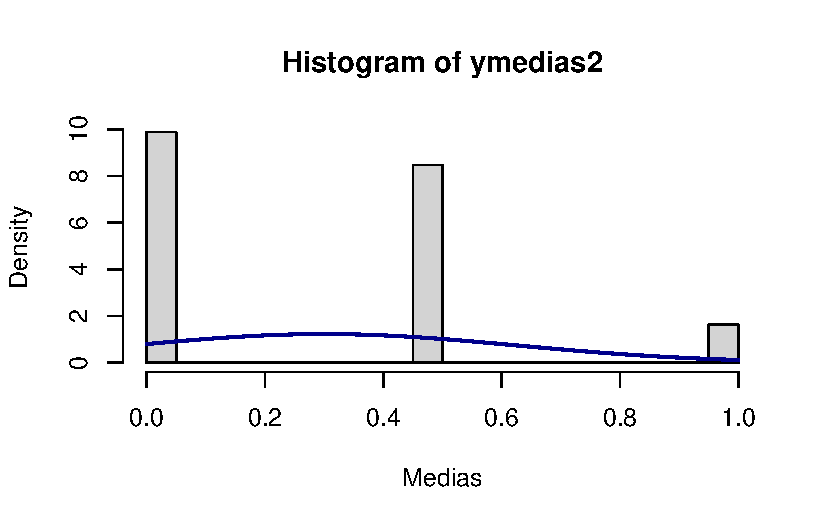
\includegraphics{tarea-1-respuestas_files/figure-pdf/unnamed-chunk-2-1.pdf}

}

\end{figure}

\emph{El histograma no se parece nada a la curva normal.}

\begin{enumerate}
\def\labelenumi{\alph{enumi}.}
\tightlist
\item
  {[}3 puntos{]} Repita lo realizado en la parte b., ahora con \(N=10\).
  Comente sobre lo que observa.
\end{enumerate}

\begin{Shaded}
\begin{Highlighting}[]
\NormalTok{reps }\OtherTok{\textless{}{-}} \DecValTok{1000}
\NormalTok{n }\OtherTok{\textless{}{-}} \DecValTok{10}
\NormalTok{p }\OtherTok{\textless{}{-}} \FloatTok{0.3}
\NormalTok{v }\OtherTok{\textless{}{-}}\NormalTok{ p}\SpecialCharTok{*}\NormalTok{(}\DecValTok{1}\SpecialCharTok{{-}}\NormalTok{p)}\SpecialCharTok{/}\NormalTok{n}

\NormalTok{ymedias10 }\OtherTok{\textless{}{-}} \FunctionTok{numeric}\NormalTok{(reps)}
\ControlFlowTok{for}\NormalTok{ (i }\ControlFlowTok{in} \DecValTok{1}\SpecialCharTok{:}\NormalTok{reps)\{}
\NormalTok{ sample }\OtherTok{\textless{}{-}} \FunctionTok{rbernoulli}\NormalTok{(n, p)}
\NormalTok{ ymedias10[i]}\OtherTok{\textless{}{-}}\FunctionTok{mean}\NormalTok{(sample)}
\NormalTok{\}}
\end{Highlighting}
\end{Shaded}

\emph{Graficamos junto con una densidad \(N(0.3, 0.21/10)\):}

\begin{Shaded}
\begin{Highlighting}[]
\FunctionTok{hist}\NormalTok{(ymedias10, }\AttributeTok{breaks=}\DecValTok{20}\NormalTok{, }\AttributeTok{prob=}\ConstantTok{TRUE}\NormalTok{)}
\FunctionTok{curve}\NormalTok{(}\FunctionTok{dnorm}\NormalTok{(x, }\AttributeTok{mean=}\NormalTok{p, }\AttributeTok{sd=}\FunctionTok{sqrt}\NormalTok{(v)), }
      \AttributeTok{col=}\StringTok{"darkblue"}\NormalTok{, }\AttributeTok{lwd=}\DecValTok{2}\NormalTok{, }\AttributeTok{add=}\ConstantTok{TRUE}\NormalTok{, }\AttributeTok{yaxt=}\StringTok{"n"}\NormalTok{)}
\end{Highlighting}
\end{Shaded}

\begin{figure}[H]

{\centering 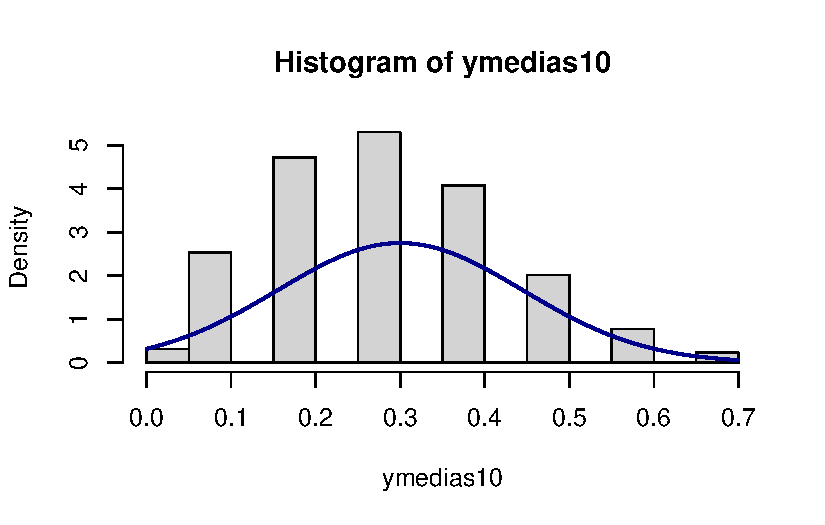
\includegraphics{tarea-1-respuestas_files/figure-pdf/unnamed-chunk-4-1.pdf}

}

\end{figure}

\emph{El histograma comienza a tener una forma normal. De hecho, se
parece ya bastante.}

\begin{enumerate}
\def\labelenumi{\alph{enumi}.}
\tightlist
\item
  {[}3 puntos{]} Repita lo realizado en la parte b., ahora con
  \(N=10,000\). Comente sobre lo que observa.
\end{enumerate}

\emph{Graficamos junto con una densidad \(N(0.3, 0.21/10000)\):}

\begin{Shaded}
\begin{Highlighting}[]
\FunctionTok{hist}\NormalTok{(ymedias10000, }\AttributeTok{breaks=}\DecValTok{20}\NormalTok{, }\AttributeTok{prob=}\ConstantTok{TRUE}\NormalTok{, }
     \AttributeTok{xlab=}\StringTok{"Medias"}\NormalTok{)}
\FunctionTok{curve}\NormalTok{(}\FunctionTok{dnorm}\NormalTok{(x, }\AttributeTok{mean=}\NormalTok{p, }\AttributeTok{sd=}\FunctionTok{sqrt}\NormalTok{(v)), }
      \AttributeTok{col=}\StringTok{"darkblue"}\NormalTok{, }\AttributeTok{lwd=}\DecValTok{2}\NormalTok{, }\AttributeTok{add=}\ConstantTok{TRUE}\NormalTok{, }\AttributeTok{yaxt=}\StringTok{"n"}\NormalTok{)}
\end{Highlighting}
\end{Shaded}

\begin{figure}[H]

{\centering 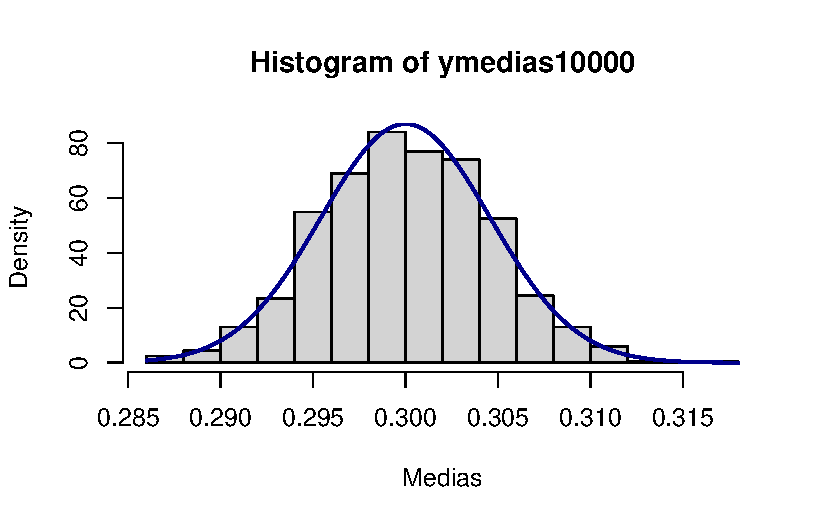
\includegraphics{tarea-1-respuestas_files/figure-pdf/unnamed-chunk-6-1.pdf}

}

\end{figure}

\emph{El histograma se parece ya a la curva normal teórica, con una
varianza muy pequeña, con la gran mayoría de las medias concentradas muy
cerca del valor esperado.}

\begin{enumerate}
\def\labelenumi{\alph{enumi}.}
\tightlist
\item
  {[}5 puntos{]} ¿Cómo usaría este ejercicio con palabras simples para
  explicar a una persona que no sabe mucho de estadística sobre la
  importancia de los teoremas de límite central?
\end{enumerate}

\emph{Un TLC nos permite hacer afirmaciones sobre la distribución de un
estadístico. Un estadístico es un resumen de los datos, por lo que nos
interesa usar dichos estadísticos para describir características de los
fenómenos que estudiamos usando datos. Queremos saber cosas como lo que
esperamos en promedio que suceda con una variable, o qué tanta
variabilidad dicha variable tendrá en la población. Con un TLC podemos
hacer afirmaciones sobre cómo lucen promedios muestrales de la variable
que estudiamos cuando tenemos suficientes observaciones. Nos dice en
particular que va a tener una distribución normal.}

\hypertarget{pregunta-5}{%
\subsection{Pregunta 5}\label{pregunta-5}}

Use los datos en el archivo \emph{motral2012.csv}, que incluye una
muestra de individuos con sus características socioeconómicas. Nos
interesa conocer los factores que afectan la probabilidad de que los
individuos tengan ahorros. Considere lo siguiente sobre las opciones de
ahorro de los entrevistados, contenida en la variable \textbf{p14}:

\begin{itemize}
\tightlist
\item
  \textbf{p14} igual a 1 significa cuentas de ahorro bancarias
\item
  \textbf{p14} igual a 2 significa cuenta de inversión bancaria
\item
  \textbf{p14} igual a 3 significa inversiones en bienes raíces
\item
  \textbf{p14} igual a 4 significa caja de ahorro en su trabajo
\item
  \textbf{p14} igual a 5 significa caja de ahorro con sus amigos
\item
  \textbf{p14} igual a 6 significa tandas
\item
  \textbf{p14} igual a 7 significa que ahorra en su casa o alcancías
\item
  \textbf{p14} igual a 8 significa otro lugar
\item
  \textbf{p14} NA significa que no ahorra
\end{itemize}

\begin{enumerate}
\def\labelenumi{\alph{enumi}.}
\tightlist
\item
  {[}2 puntos{]} Comience generando una variable binaria \textbf{ahorra}
  que tome el valor de 1 para las personas que ahorran y 0 en otro caso.
  Construya también la variable \textbf{mujer} que tome el valor de 1
  cuando \textbf{sex} toma el valor de 2 y 0 en otro caso.
\end{enumerate}

\emph{Generamos variables:}

\begin{Shaded}
\begin{Highlighting}[]
\NormalTok{data.financiero }\OtherTok{\textless{}{-}} \FunctionTok{read\_csv}\NormalTok{(}\StringTok{"../files/motral2012.csv"}\NormalTok{,}
                          \AttributeTok{locale =} \FunctionTok{locale}\NormalTok{(}\AttributeTok{encoding =} \StringTok{"latin1"}\NormalTok{)) }\SpecialCharTok{\%\textgreater{}\%}
  \FunctionTok{clean\_names}\NormalTok{() }\SpecialCharTok{\%\textgreater{}\%} 
  \FunctionTok{mutate}\NormalTok{(}\AttributeTok{ahorra =} \FunctionTok{ifelse}\NormalTok{(}\FunctionTok{is.na}\NormalTok{(p14), }\DecValTok{0}\NormalTok{, }\DecValTok{1}\NormalTok{),}
         \AttributeTok{mujer=}\FunctionTok{ifelse}\NormalTok{(sex}\SpecialCharTok{==}\DecValTok{2}\NormalTok{,}\DecValTok{1}\NormalTok{,}\DecValTok{0}\NormalTok{))}
\end{Highlighting}
\end{Shaded}

\begin{enumerate}
\def\labelenumi{\alph{enumi}.}
\tightlist
\item
  {[}3 puntos{]} Estime un modelo de probabilidad lineal que relacione
  \textbf{ahorra} como variable dependiente con \textbf{eda} (edad),
  \textbf{anios\_esc} (años de escolaridad) y \textbf{mujer}. Reporte
  los errores que asumen homocedasticidad y los errores robustos a
  heteroscedasticidad.
\end{enumerate}

\emph{Estimamos el modelo lineal y obtenemos la matriz de varianzas
robusta usando vcovHC:}

\begin{Shaded}
\begin{Highlighting}[]
\FunctionTok{summary}\NormalTok{(reg.lineal }\OtherTok{\textless{}{-}} \FunctionTok{lm}\NormalTok{(ahorra }\SpecialCharTok{\textasciitilde{}}\NormalTok{ eda }\SpecialCharTok{+}\NormalTok{ anios\_esc }\SpecialCharTok{+}\NormalTok{ mujer,}
                         \AttributeTok{data =}\NormalTok{ data.financiero))}
\end{Highlighting}
\end{Shaded}

\begin{verbatim}

Call:
lm(formula = ahorra ~ eda + anios_esc + mujer, data = data.financiero)

Residuals:
    Min      1Q  Median      3Q     Max 
-1.9816 -0.4626 -0.2984  0.4947  0.8254 

Coefficients:
              Estimate Std. Error t value Pr(>|t|)    
(Intercept)  0.4559531  0.0303390  15.029  < 2e-16 ***
eda         -0.0049494  0.0006541  -7.567  4.5e-14 ***
anios_esc    0.0174601  0.0014516  12.028  < 2e-16 ***
mujer       -0.0140326  0.0134973  -1.040    0.299    
---
Signif. codes:  0 '***' 0.001 '**' 0.01 '*' 0.05 '.' 0.1 ' ' 1

Residual standard error: 0.4892 on 5260 degrees of freedom
Multiple R-squared:  0.04033,   Adjusted R-squared:  0.03978 
F-statistic: 73.69 on 3 and 5260 DF,  p-value: < 2.2e-16
\end{verbatim}

\begin{Shaded}
\begin{Highlighting}[]
\CommentTok{\#Matriz robusta}
\NormalTok{v\_rob }\OtherTok{\textless{}{-}} \FunctionTok{vcovHC}\NormalTok{(reg.lineal, }\AttributeTok{type =} \StringTok{"HC0"}\NormalTok{)}
\NormalTok{se\_rob    }\OtherTok{\textless{}{-}} \FunctionTok{sqrt}\NormalTok{(}\FunctionTok{diag}\NormalTok{(v\_rob))}
\end{Highlighting}
\end{Shaded}

\emph{Presentamos usando stargazer, aunque pueden usar el paquete de su
preferencia. Por ejemplo, quizás quieran darle una revisada a
modelsummary.}

Dependent variable:

ahorra

(1)

(2)

eda

-0.0049***

-0.0049***

(0.0007)

(0.0007)

anios\_esc

0.0175***

0.0175***

(0.0015)

(0.0024)

mujer

-0.0140

-0.0140

(0.0135)

(0.0135)

Constant

0.4560***

0.4560***

(0.0303)

(0.0385)

Observations

5,264

5,264

R2

0.0403

0.0403

Adjusted R2

0.0398

0.0398

Residual Std. Error (df = 5260)

0.4892

0.4892

F Statistic (df = 3; 5260)

73.6878***

73.6878***

Note:

\emph{p\textless0.1; \textbf{p\textless0.05; }}p\textless0.01

\begin{enumerate}
\def\labelenumi{\alph{enumi}.}
\tightlist
\item
  {[}3 puntos{]} ¿Cuál es el efecto en la probabilidad de ahorrar si los
  años de educación se incrementan en una unidad, pasando de 3 a 4 años
  de educación?
\end{enumerate}

\emph{En un modelo lineal esto es simplemente un incremento en 1.75
puntos porcentuales.}

\begin{enumerate}
\def\labelenumi{\alph{enumi}.}
\tightlist
\item
  {[}4 puntos{]} Realice una prueba de significancia conjunta de
  \textbf{eda} y \textbf{anios\_esc}. ¿Qué concluye?
\end{enumerate}

\emph{Podemos usar la función linearHypothesis:}

\begin{Shaded}
\begin{Highlighting}[]
\NormalTok{car}\SpecialCharTok{::}\FunctionTok{linearHypothesis}\NormalTok{(reg.lineal, }\FunctionTok{c}\NormalTok{(}\StringTok{"eda=0"}\NormalTok{, }\StringTok{"anios\_esc=0"}\NormalTok{))}
\end{Highlighting}
\end{Shaded}

\begin{verbatim}
Linear hypothesis test

Hypothesis:
eda = 0
anios_esc = 0

Model 1: restricted model
Model 2: ahorra ~ eda + anios_esc + mujer

  Res.Df    RSS Df Sum of Sq      F    Pr(>F)    
1   5262 1311.5                                  
2   5260 1258.9  2    52.597 109.88 < 2.2e-16 ***
---
Signif. codes:  0 '***' 0.001 '**' 0.01 '*' 0.05 '.' 0.1 ' ' 1
\end{verbatim}

\emph{Concluimos que no hay evidencia para afirmar que
\(\beta_{eda}=\beta_{anios\_esc}=0\).}

\begin{enumerate}
\def\labelenumi{\alph{enumi}.}
\tightlist
\item
  {[}4 puntos{]} Estime un modelo probit relacionando las mismas
  variables. Use la función \emph{avg\_slopes} del paquete
  \emph{marginaleffects} para obtener los efectos marginales promedio de
  un cambio en cada uno de los regresores. ¿Por qué difiere la magnitud
  de este efecto marginal con respecto a la parte c.?
\end{enumerate}

\emph{Estimamos el modelo probit:}

\begin{Shaded}
\begin{Highlighting}[]
\NormalTok{reg.probit }\OtherTok{\textless{}{-}} \FunctionTok{glm}\NormalTok{(ahorra }\SpecialCharTok{\textasciitilde{}}\NormalTok{ eda }\SpecialCharTok{+}\NormalTok{ anios\_esc }\SpecialCharTok{+}\NormalTok{ mujer,}
                  \AttributeTok{family =} \FunctionTok{binomial}\NormalTok{(}\AttributeTok{link =} \StringTok{"probit"}\NormalTok{),}
                  \AttributeTok{data =}\NormalTok{ data.financiero)}

\FunctionTok{summary}\NormalTok{(reg.probit)}\SpecialCharTok{$}\NormalTok{coef}
\end{Highlighting}
\end{Shaded}

\begin{verbatim}
               Estimate  Std. Error   z value     Pr(>|z|)
(Intercept) -0.18770947 0.083351859 -2.252013 2.432145e-02
eda         -0.01258123 0.001703646 -7.384884 1.525863e-13
anios_esc    0.05130108 0.004480285 11.450404 2.340518e-30
mujer       -0.04077164 0.035053348 -1.163131 2.447763e-01
\end{verbatim}

\emph{Noten que el signo de los coeficientes coinciden con el promedio
de los efectos marginales:}

\begin{Shaded}
\begin{Highlighting}[]
\FunctionTok{avg\_slopes}\NormalTok{(reg.probit)}
\end{Highlighting}
\end{Shaded}

\begin{verbatim}

      Term Contrast Estimate Std. Error     z Pr(>|z|)     S    2.5 %   97.5 %
 anios_esc    dY/dX  0.01977   0.001659 11.91   <0.001 106.3  0.01651  0.02302
 eda          dY/dX -0.00485   0.000646 -7.51   <0.001  43.9 -0.00611 -0.00358
 mujer        1 - 0 -0.01571   0.013504 -1.16    0.245   2.0 -0.04218  0.01076

Columns: term, contrast, estimate, std.error, statistic, p.value, s.value, conf.low, conf.high 
\end{verbatim}

\emph{El promedio del efecto marginal de un cambio en los años de
educación es de 2 puntos porcentuales. Ligeramente superior al efecto
obtenido en el modelo lineal.}

\begin{enumerate}
\def\labelenumi{\alph{enumi}.}
\tightlist
\item
  {[}4 puntos{]} Ahora estime el efecto marginal en la media para
  \textbf{eda} y \textbf{anios\_esc} y para las mujeres, usando la
  función \emph{slopes}. ¿Por qué difiere la magnitud de este efecto
  marginal respecto a la parte c.~y la d.?
\end{enumerate}

\emph{Para obtener los efectos marginales evaluados en algun valor
\(X_i\) de los covariables, debemos especificar estos valores usando
datagrid:}

\begin{Shaded}
\begin{Highlighting}[]
\FunctionTok{avg\_slopes}\NormalTok{(reg.probit,}
           \AttributeTok{newdata =} \FunctionTok{datagrid}\NormalTok{(}\AttributeTok{eda =} \FunctionTok{mean}\NormalTok{(data.financiero}\SpecialCharTok{$}\NormalTok{eda),}
                              \AttributeTok{anios\_esc =} \FunctionTok{mean}\NormalTok{(data.financiero}\SpecialCharTok{$}\NormalTok{anios\_esc),}
                              \AttributeTok{mujer =} \DecValTok{1}\NormalTok{))}
\end{Highlighting}
\end{Shaded}

\begin{verbatim}

      Term Contrast Estimate Std. Error     z Pr(>|z|)    S    2.5 %   97.5 %
 anios_esc    dY/dX   0.0204   0.001779 11.46   <0.001 98.5  0.01689  0.02386
 eda          dY/dX  -0.0050   0.000677 -7.38   <0.001 42.5 -0.00632 -0.00367
 mujer        1 - 0  -0.0162   0.013944 -1.16    0.245  2.0 -0.04355  0.01111

Columns: term, contrast, estimate, std.error, statistic, p.value, s.value, conf.low, conf.high 
\end{verbatim}

\emph{El efecto marginal de un cambio en los años de escolaridad
evaluados en la media de los años de educación y edad, para las mujeres,
es de 2.04 puntos. Esto difiere del modelo lineal porque en el modelo
lineal los efectos marginales son constantes, mientras que los efectos
marginal del modelo no lineal dependen del punto de evaluación. También
difiere de los efectos marginales promedio pues aquí solo hemos
calculado el efecto marginal una sola vez, para un valor \(X_i\),
mientras que el promedio de efectos marginales implica calcular el
efecto marginal para cada individuo y luego obtener el promedio.}

\emph{En clase les pregunté cómo estimarían el error estándar de los
cambios marginales y brevemente mencioné que una forma muy usada es el
Método Delta, el cual se basa en que los efectos marginales son
funciones no lineales de los parámetros. Esto es lo que efectivamente se
usa en la función avg\_slopes para obtener los errores estándar y los
intervalos de confianza.
\href{https://marginaleffects.com/articles/uncertainty.html}{Aquí}
pueden leer al respecto.}

\hypertarget{pregunta-6}{%
\subsection{Pregunta 6}\label{pregunta-6}}

Ahora estimará un modelo multinomial empleando los mismos datos en
\emph{motral2012.csv}. El propósito será ahora estudiar los factores
relevantes para predecir la forma de ahorro que tienen las personas que
ahorran.

\begin{enumerate}
\def\labelenumi{\alph{enumi}.}
\tightlist
\item
  {[}2 punto{]} Genere una variable categórica llamada \textbf{ahorro}
  que sea igual a 1 cuando \textbf{p14} sea igual a 1 o 2, igual a 2
  cuando \textbf{p14} sea igual a 7, e igual a 3 cuando \textbf{p14} sea
  igual a 3, 4, 5, 6 u 8. Haga que esa variable sea missing cuando
  \textbf{p14} sea missing. Posteriormente, convierta esta nueva
  variable en una de factores de forma que el valor 1 tenga la etiqueta
  ``Banco'', el valor 2 tenga la etiqueta ``Casa'' y el valor 3 tenga la
  etiqueta ``Otro''.
\end{enumerate}

\emph{Construimos la variable dependiente:}

\begin{Shaded}
\begin{Highlighting}[]
\NormalTok{data.financiero }\OtherTok{\textless{}{-}} \FunctionTok{read\_csv}\NormalTok{(}\StringTok{"../files/motral2012.csv"}\NormalTok{,}
                            \AttributeTok{locale =} \FunctionTok{locale}\NormalTok{(}\AttributeTok{encoding =} \StringTok{"latin1"}\NormalTok{)) }\SpecialCharTok{\%\textgreater{}\%}
  \FunctionTok{clean\_names}\NormalTok{() }\SpecialCharTok{\%\textgreater{}\%} 
  \FunctionTok{mutate}\NormalTok{(}\AttributeTok{ahorro=}\ConstantTok{NA}\NormalTok{) }\SpecialCharTok{\%\textgreater{}\%} 
  \FunctionTok{mutate}\NormalTok{(}\AttributeTok{ahorro=}\FunctionTok{ifelse}\NormalTok{(p14}\SpecialCharTok{\%in\%}\FunctionTok{c}\NormalTok{(}\DecValTok{1}\NormalTok{,}\DecValTok{2}\NormalTok{),}\DecValTok{1}\NormalTok{,ahorro)) }\SpecialCharTok{\%\textgreater{}\%}
  \FunctionTok{mutate}\NormalTok{(}\AttributeTok{ahorro=}\FunctionTok{ifelse}\NormalTok{(p14}\SpecialCharTok{==}\DecValTok{7}\NormalTok{,}\DecValTok{2}\NormalTok{,ahorro)) }\SpecialCharTok{\%\textgreater{}\%} 
  \FunctionTok{mutate}\NormalTok{(}\AttributeTok{ahorro=}\FunctionTok{ifelse}\NormalTok{(p14}\SpecialCharTok{\%in\%}\FunctionTok{c}\NormalTok{(}\DecValTok{3}\NormalTok{,}\DecValTok{4}\NormalTok{,}\DecValTok{5}\NormalTok{,}\DecValTok{6}\NormalTok{,}\DecValTok{8}\NormalTok{),}\DecValTok{3}\NormalTok{,ahorro)) }\SpecialCharTok{\%\textgreater{}\%} 
  \FunctionTok{mutate}\NormalTok{(}\AttributeTok{ahorro=}\FunctionTok{factor}\NormalTok{(ahorro,}
                   \AttributeTok{levels=}\FunctionTok{c}\NormalTok{(}\DecValTok{1}\NormalTok{,}\DecValTok{2}\NormalTok{,}\DecValTok{3}\NormalTok{), }\AttributeTok{labels=}\FunctionTok{c}\NormalTok{(}\StringTok{"Banco"}\NormalTok{,}\StringTok{"Casa"}\NormalTok{,}\StringTok{"Otro"}\NormalTok{))) }\SpecialCharTok{\%\textgreater{}\%}
  \FunctionTok{mutate}\NormalTok{(}\AttributeTok{mujer=}\FunctionTok{ifelse}\NormalTok{(sex}\SpecialCharTok{==}\DecValTok{2}\NormalTok{,}\DecValTok{1}\NormalTok{,}\DecValTok{0}\NormalTok{))}
\end{Highlighting}
\end{Shaded}

\begin{enumerate}
\def\labelenumi{\alph{enumi}.}
\tightlist
\item
  {[}4 puntos{]} Estime un modelo logit multinomial (regresores
  invariantes a la alternativa) con la opción de ahorro como variable
  dependiente y los mismos regresores de la pregunta 5. Hay varios
  paquetes para hacer esto, pero recomiendo usar la función
  \emph{multinom} del paquete \emph{nnet}. ¿Qué puede decir sobre el
  coeficiente de años de educación en la alternativa ``Casa''?
\end{enumerate}

\emph{Usamos multinom para estimar el modelo logit multinomial:}

\begin{Shaded}
\begin{Highlighting}[]
\NormalTok{multilogit }\OtherTok{\textless{}{-}}\NormalTok{ nnet}\SpecialCharTok{::}\FunctionTok{multinom}\NormalTok{(ahorro}\SpecialCharTok{\textasciitilde{}}\NormalTok{ eda }\SpecialCharTok{+}\NormalTok{ anios\_esc }\SpecialCharTok{+}\NormalTok{ mujer,}
                              \AttributeTok{data=}\NormalTok{data.financiero)}
\end{Highlighting}
\end{Shaded}

\begin{verbatim}
# weights:  15 (8 variable)
initial  value 2727.854313 
iter  10 value 2546.085070
final  value 2545.712541 
converged
\end{verbatim}

\begin{Shaded}
\begin{Highlighting}[]
\FunctionTok{summary}\NormalTok{(multilogit)}
\end{Highlighting}
\end{Shaded}

\begin{verbatim}
Call:
nnet::multinom(formula = ahorro ~ eda + anios_esc + mujer, data = data.financiero)

Coefficients:
     (Intercept)          eda   anios_esc       mujer
Casa    3.026880 -0.052310196 -0.14829719  0.09265405
Otro    0.206704 -0.003501367 -0.04628175 -0.06459305

Std. Errors:
     (Intercept)         eda  anios_esc      mujer
Casa   0.2487107 0.005207439 0.01355319 0.09956544
Otro   0.2476498 0.004964123 0.01285100 0.09995715

Residual Deviance: 5091.425 
AIC: 5107.425 
\end{verbatim}

\emph{En el logit multinominal (regresores invariantes) el coeficiente
se interpreta con respecto a una categoría base. En este caso, la
categoría base es Banco. El modelo implica que la probabilidad de
ahorrar en casa disminuye con un año más de educación, en comparación
con la probabilidad de ahorrar en el banco. En particular, sabemos que
podemos escribir el log del cociente de la probabilidad de las
categorías \(j\) y \(k\) sean escogidas, normalizando \(k\) a ser la
base, como:}

\[\ln\left(\frac{P(y=Casa)}{P(y=Banco)}\right)=x'\beta=\beta_0+\beta_1 edad + \beta_2 educación + \beta_3 mujer \]

\emph{Ees decir, un año más de educación se asocia con una reducción en
el log de la razón de momios de 0.15.}

\begin{enumerate}
\def\labelenumi{\alph{enumi}.}
\tightlist
\item
  {[}6 puntos{]} Calcule los efectos marginales promedio sobre la
  probabilidad de ahorrar en el banco. Al considerar el cambio en la
  probabilidad para el caso de las mujeres (cuando la variable
  \textbf{mujer} pasa de 0 a 1), ¿de qué tamaño es el efecto predicho en
  la probabilidad de ahorrar en el banco?
\end{enumerate}

\emph{Usamos avg\_slopes}:

\begin{Shaded}
\begin{Highlighting}[]
\FunctionTok{avg\_slopes}\NormalTok{(multilogit)}
\end{Highlighting}
\end{Shaded}

\begin{verbatim}

 Group      Term Contrast Estimate Std. Error       z Pr(>|z|)    S    2.5 %
 Banco anios_esc    dY/dX  0.02285   0.002381   9.595   <0.001 70.0  0.01818
 Banco eda          dY/dX  0.00657   0.000935   7.027   <0.001 38.8  0.00474
 Banco mujer        1 - 0 -0.00343   0.019432  -0.177    0.860  0.2 -0.04152
 Casa  anios_esc    dY/dX -0.02512   0.002231 -11.262   <0.001 95.3 -0.02949
 Casa  eda          dY/dX -0.00982   0.000860 -11.422   <0.001 98.0 -0.01151
 Casa  mujer        1 - 0  0.02271   0.017662   1.286    0.199  2.3 -0.01191
 Otro  anios_esc    dY/dX  0.00228   0.002174   1.046    0.295  1.8 -0.00199
 Otro  eda          dY/dX  0.00325   0.000842   3.863   <0.001 13.1  0.00160
 Otro  mujer        1 - 0 -0.01927   0.017549  -1.098    0.272  1.9 -0.05367
   97.5 %
  0.02751
  0.00840
  0.03465
 -0.02075
 -0.00814
  0.05732
  0.00654
  0.00490
  0.01512

Columns: term, group, contrast, estimate, std.error, statistic, p.value, s.value, conf.low, conf.high 
\end{verbatim}

\emph{El efecto de ser mujer es de un incremento de apenas 0.3 puntos en
la probabilidad de ahorrar en el banco al estimar el promedio de los
efectos marginales.}

\begin{enumerate}
\def\labelenumi{\alph{enumi}.}
\tightlist
\item
  {[}4 puntos{]} Calcule los cocientes de riesgo relativo
  (\emph{relative risk ratios} o RRR). ¿Qué significa el hecho de que el
  RRR asociado a ser mujer sea mayor que 1 en la alternativa ``Casa''?
\end{enumerate}

\begin{Shaded}
\begin{Highlighting}[]
\NormalTok{(}\AttributeTok{multilogit\_rrr =} \FunctionTok{exp}\NormalTok{(}\FunctionTok{coef}\NormalTok{(multilogit)))}
\end{Highlighting}
\end{Shaded}

\begin{verbatim}
     (Intercept)       eda anios_esc     mujer
Casa   20.632752 0.9490344 0.8621748 1.0970821
Otro    1.229619 0.9965048 0.9547729 0.9374489
\end{verbatim}

\emph{Los coeficientes en forma de RRR tienen la interpretación del
cambio en el riesgo relativo que una categoría sea elegida con relación
al riesgo de escoger la categoría base. En este caso, el ser mujer está
asociado con una probabilidad de ahorrar en ``Casa'' 1.097 veces mayor
de que la de ahorrar en ``Banco''.}

\begin{enumerate}
\def\labelenumi{\alph{enumi}.}
\tightlist
\item
  {[}4 puntos{]} Estime nuevamente el modelo, pero ahora, especifique
  que la alternativa ``Casa'' sea la alternativa base. ¿Cómo es el RRR
  de la edad en la alternativa ``Banco''? ¿Es esto congruente con lo que
  obtuvo en la parte d.~de esta pregunta?
\end{enumerate}

\emph{Primero tenemos que cambiar la base. Para esto hacemos uso de que
ahorro es una variable de factores. Luego estimamos:}

\begin{Shaded}
\begin{Highlighting}[]
\NormalTok{data.financiero }\OtherTok{\textless{}{-}}\NormalTok{ data.financiero }\SpecialCharTok{\%\textgreater{}\%} 
  \FunctionTok{mutate}\NormalTok{(}\AttributeTok{ahorro =} \FunctionTok{relevel}\NormalTok{(ahorro, }\AttributeTok{ref =} \StringTok{"Casa"}\NormalTok{))}

\NormalTok{multilogit2 }\OtherTok{\textless{}{-}}\NormalTok{ nnet}\SpecialCharTok{::}\FunctionTok{multinom}\NormalTok{(ahorro }\SpecialCharTok{\textasciitilde{}}\NormalTok{ eda }\SpecialCharTok{+}\NormalTok{ anios\_esc }\SpecialCharTok{+}\NormalTok{ mujer,}
                              \AttributeTok{data=}\NormalTok{data.financiero)}
\end{Highlighting}
\end{Shaded}

\begin{verbatim}
# weights:  15 (8 variable)
initial  value 2727.854313 
iter  10 value 2552.696634
final  value 2545.712541 
converged
\end{verbatim}

\begin{Shaded}
\begin{Highlighting}[]
\NormalTok{(}\AttributeTok{multilogit2\_rrr =} \FunctionTok{exp}\NormalTok{(}\FunctionTok{coef}\NormalTok{(multilogit2)))}
\end{Highlighting}
\end{Shaded}

\begin{verbatim}
      (Intercept)      eda anios_esc     mujer
Banco  0.04846638 1.053703  1.159857 0.9115111
Otro   0.05959489 1.050020  1.107401 0.8544952
\end{verbatim}

\emph{Obtenemos el RRR:}

\begin{Shaded}
\begin{Highlighting}[]
\NormalTok{(}\AttributeTok{mmultilogit\_rrr =} \FunctionTok{exp}\NormalTok{(}\FunctionTok{coef}\NormalTok{(multilogit)))}
\end{Highlighting}
\end{Shaded}

\begin{verbatim}
     (Intercept)       eda anios_esc     mujer
Casa   20.632752 0.9490344 0.8621748 1.0970821
Otro    1.229619 0.9965048 0.9547729 0.9374489
\end{verbatim}

\emph{Al cambiar la categoría base a Casa solo se modifica la
interpretación relativa. En la parte d.~el RRR de la edad para la opción
de Casa era 0.949, es decir, si la edad se incrementa en una unidad, la
probabilidad de ahorrar en Casa es 0.949 veces la de ahorrar en Banco.
Con la nueva categoría base, el RRR de la edad para ahorrar en Banco es
1.054, es decir, si la edad se incrementa en un año, la probabilidad de
ahorrar en Banco es 1.054 veces más probable que la probabilidad de
ahorrar en Casa. La parte d.~implica que \(P(Casa)=0.949(Banco)\).
Mientras que estimando el modelo con la nueva categoría,
\(P(Banco)=1.054(Casa)\), o \(P(Casa)=1/1.054(Banco)\). Empleando todos
los decimales en R se puede notar que 1/1.054≅0.949 Ambos resultados son
consistentes.}



\end{document}
